%
% Revision 30 Nov 2023
%
%%%%%%%%%%%%%%%%%%%%%%%%%%%%%%%%%%%%%%%%%%%%%%%%%%%%%%%%%%%%%%%%%%%%%%%%%%%%%%%%
%2345678901234567890123456789012345678901234567890123456789012345678901234567890
%        1         2         3         4         5         6         7         8
% DOCUMENT CLASS
\documentclass[a4paper,12pt]{Classes/RoboticsLaTeX}

% USEFUL PACKAGES
% Commonly-used packages are included by default.
% Refer to section "Book - Useful packages" in the class file "Classes/RoboticsLaTeX.cls" for the complete list.
\usepackage{amsmath}
\usepackage{amsfonts}
\usepackage{algorithm}
\usepackage{algorithmic}
\usepackage{multirow}
\usepackage{colortbl}
\usepackage{color}
\usepackage[table]{xcolor}
\usepackage{epigraph}
\usepackage{graphicx}
%\usepackage{subfigure}
\usepackage{caption}
\usepackage{subcaption}
\usepackage{hyperref}
\usepackage{tabularx}
\usepackage{float}
\usepackage{longtable}
\usepackage[pdftex]{graphicx}
\usepackage{pdfpages}
\usepackage{pdflscape}
\usepackage[acronym,toc]{glossaries}
\usepackage{setspace}
\usepackage[utf8]{inputenc}
\usepackage[table]{xcolor}

%\usepackage{layout}

\setstretch{1.5}
%\onehalfspacing

% SPECIAL COMMANDS
% correct bad hyphenation
\hyphenation{op-tical net-works semi-conduc-tor}
\hyphenation{par-ti-cu-lar mo-du-le ge-stu-re}
% INTERLINEA 1.5
%\renewcommand{\baselinestretch}{1.5}

%% ignore slightly overfull and underfull boxes
%\hbadness=10000
%\hfuzz=50pt
% declare commonly used operators
%\DeclareMathOperator*{\argmax}{argmax}

% >>>> Replace all the [[Placeholders]] on the front page and in the Declaration <<<<

\title{\Large{Cycleway and Road Quality Analytics using IMU Sensor and Artificial Intelligence}}

\author{SHARAJ JAGADEESAN}
\collegeordept{School of Computer Science}
\university{University of Galway}
\crest{
\includegraphics[width=135mm]{Figures/University_Of_Galway_Logo__Positive_Landscape.png}}
%\crest{
\includegraphics[width=80mm]{Figures/University_of_Galway_logo_2022.png}}

\supervisor{Waqar Shahid Qureshi}
%\supervisor{Name of the Supervisor}
%\supervisor{Name of the Co-Supervisor}	

% replace NAME with your name and PROGRAMME with Data Analytics, Artificial Intelligence, or Artificial Intelligence - Online
\degree{MSc in Computer Science (Data Analytics)}
\degreedate{21 August 2024}  % Replace with submission date


%%%%%%%%%%%%%%%%%%%%%%%%%%%%%%%%%%%%%%%%%%%%%%%%%%%%%%%%%%%%%%%%%%%%%%%%%%%%%%%%
%%% uncomment if glossary needed, see examples in file
%\makeglossaries
%\loadglsentries{glossary}

\begin{document}
	\begin{spacing}{1}
		\maketitle
	\end{spacing}
	
	% add an empty page after title page
	\newpage\null\thispagestyle{empty}\newpage
	
	% set the number of sectioning levels that get number and appear in the contents
	\setcounter{secnumdepth}{3}
	\setcounter{tocdepth}{3}
	
	\frontmatter
	
	% Replace NAME and THESIS-TITLE with your name and the title of this thesis.
	\textbf{DECLARATION} 
	I, SHARAJ JAGADEESAN, hereby declare that this thesis, titled ``Cycleway and Road Quality Analytics using IMU Sensor and Artificial Intelligence'', and the work presented in it are entirely my own except where explicitly stated otherwise in the text, and that this work has not been previously submitted, in part or whole, to any university or institution for any degree, diploma, or other qualification. 
	\newline
	
	\begin{tabular}{@{}p{.5in}p{4in}@{}}
		Signature: & ~~\hrulefill \\
	\end{tabular}
	\newpage
	
	
	%%%% uncomment if acknowledgements needed
	%\textbf{Acknowledgement}
	%
	%
	%\newpage\textbf{}
	
	
	% THESIS ABSTRACT
	\begin{abstracts}
		Enhancing cycleway infrastructure requires effective analysis of the road quality for sustainability, user satisfaction, and environmental preservation. This project addresses the challenge of identifying and classifying road infrastructure and elements related to cyclists by developing an index to measure cycleway and road quality. Leveraging advancements in data analytics and machine learning, we propose a comprehensive data analytics tool tailored for cycleway and road quality analysis. This tool provides detailed insights into cycleway road conditions based on IMU sensor data and leveraging the power of Artificial Intelligence, benefiting cyclists by improving safety and navigation, and aiding road development agencies through efficient strategic planning and optimal resource allocation. The robust functionality and user-friendly interface of this solution aim to create safer and more accessible urban landscapes. By tracking road wear and tear, our method enables rapid response to infrastructure issues, ensuring the continuous quality of cycleways and roads.
		
		\textbf{Keywords: } Cycleway, Road Quality Index, Machine Learning, Neural Networks, IMU sensor, Road Development 
	
	
	\tableofcontents
	\listoffigures
	\listoftables
	\printglossary[title=List of Acronyms,type=\acronymtype]
		
	
	\mainmatter
	
	
	\chapter{Introduction}
	\label{chap:introduction}
	
Enhancing cycleway infrastructure requires robust data about the cycleways and active travel routes to ensure sustainability, user satisfaction, and environmental preservation. This project tackles the critical problem of precisely identifying and classifying road infrastructure related to cyclists by streamlining and developing an index to measure cycleway and road quality \cite{Qureshi}. The motivation for this project stems from the necessity of efficient IMU data analysis and visualization, which are crucial for both road development authorities and cyclists. The project belongs to the data analytics (DA) and artificial intelligence (AI) research areas \cite{Ranyal}, focusing on applying these technologies to improve infrastructure management. While existing research has primarily addressed general road quality monitoring \cite{Mahlberg}, there is a significant gap in tailored solutions for cycleway infrastructure. This project aims to fill this gap by leveraging advancements in data analytics and machine learning technologies, such as YOLO (You Only Look Once) object detection and IMU sensor data, to develop a comprehensive data analytics tool for cycleway road quality.

Developing or using advanced sensors for this task is expensive and not feasible in the long run. Therefore, alternative approaches need to be explored where we can utilize less expensive and easily available methods to collect data. Nowadays, all the smartphones are equipped with IMU sensors which can carry out this task \cite{Sattar}. Smartphones can be effectively utilized to capture data from different sensors and camera which can be analysed. By facilitating the input of multiple sensory inputs including videos and images, featuring road infrastructure and assets related to cyclists, the software will conduct a comprehensive statistical analysis of these cycleway, visualized through an intuitive graphical user interface. The software will also assess road quality based on IMU sensor inputs and artificial intelligence and provide a quality index for the road or cycleway, highlighting the segments of the cycleway which needs attention. This capability benefits cyclists by improving safety and navigation and aids road development agencies through efficient strategic planning and optimal resource allocation.

The project aims to answer the following research questions: How can data analytics and machine learning be applied to enhance cycleway and road quality? How can an index be developed to measure cycleway and road quality accurately? How can this tool improve safety and navigation for cyclists in urban environments? 

By providing thorough insights into road conditions, this project ultimately leads to safer and more accessible urban landscapes. The robust functionality and user-friendly interface of this solution offer a practical means of meeting the needs of road development authorities and cyclists, ensuring the continuous quality of cycleways and roads through proactive, predictive, and precise analytics.


	\chapter{Data}
	\label{chap:data}
	
	The data for this project was collected through a smartphone application called - Sensor Logger \cite{Sensorlogger}. The application provides an easy to use interface to capture accelerometer, location and video data. The smartphone is mounted on a bicycle at a fixed position and the data is captured along a 30 minutes ride. The collected data is then pre-processed to remove any noise \cite{Sattar} and processed for further analysis.

 \begin{figure}[H]
\centering
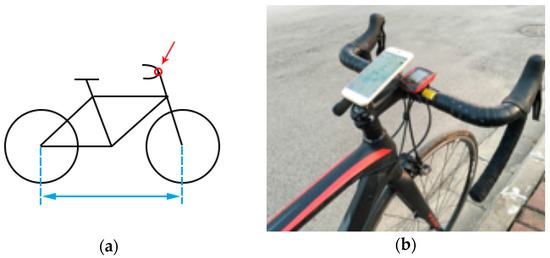
\includegraphics[width=\linewidth]{Figures/position_on_cycle.jpg}
\caption{Smartphone mounted on the bicycle for data collection from \cite{Zang}}
\label{fig:cycle}
\end{figure}

    Utilising low pass filters or high pass filters are some of the common methods used \cite{Sebestyen}. The data which we obtain from different sensors is then merged and the numbers of seconds elapsed is used as an index.

    

 
	\chapter{Methodology}
	\label{chap:methodology} 
	
	Our project is designed to enhance the planning and development of cycling infrastructure and road systems through the use of innovative IMU data analysis and visualization techniques. The data we use includes inputs from IMU sensors (Accelerometer, GPS) embedded in a smartphone, alongside video footage \cite{Zang}. The smartphone, mounted on a bicycle, captures real-time data as the bicycle navigates various roads. This data is appropriate for several reasons:

\textbf{Relevance:} The IMU sensors provide critical real-time data on the bicycle’s movement and orientation, essential for assessing road quality and detecting surface anomalies.
\vspace{10pt}

\textbf{Accessibility:} Smartphones are widely available and come with high-precision sensors, making this an affordable and scalable solution.
\vspace{10pt}

\textbf{Comprehensive Coverage:} The combination of video footage with sensor data offers a detailed view of road conditions, capturing both visual and physical aspects of the road environment.
\vspace{10pt}

This approach ensures that the data accurately represents real-world cycling conditions, providing a solid foundation for analysis.

The collected sensor data and video inputs undergo pre-processing using Python libraries such as Pandas and PIL. During pre-processing, noise is effectively filtered out to ensure the accuracy of subsequent analyses. The clean data is then fed into machine learning algorithms and neural networks, where we implement YOLO (You Only Look Once) for object detection \cite{Pham} on the video footage. This step identifies and labels various road assets and conditions.

\textbf{Pre-processing:} Python libraries such as Pandas and PIL are used for data cleaning and Scipy is used for noise filtering, which are essential for accurate data analysis.

\vspace{10pt}

\textbf{Object Detection:} YOLO is employed for its speed and accuracy in real-time video processing, allowing efficient identification and labeling of road assets and conditions \cite{Dewi}.

\vspace{10pt}

\textbf{Statistical Analysis:} The cleaned data is analyzed using Pandas to generate comprehensive statistical insights. 

\vspace{10pt}

These methods are chosen for their robustness and efficiency in handling large datasets. However, potential limitations include environmental factors affecting sensor data accuracy and the computational intensity of real-time video processing.

\vspace{10pt}

\textbf{Python Libraries:} Pandas and PIL are extensively used for data manipulation and image processing, respectively. Libraries like Plotly, Seaborn and Matplotlib are used for visualization. Libraries like Keras and Tensorflow are used for Deep Learning. Flask is used for creating a web application and Folium is used to visualise the map. These libraries are well-suited for managing large datasets and conducting detailed analyses.
These tools and algorithms were selected based on their effectiveness in handling the specific requirements of our project, such as real-time processing and high accuracy in detection and analysis.

\vspace{10pt}

How can data analytics and machine learning be applied to enhance cycleway and road quality?

By collecting and pre-processing data from IMU sensors and video footage, and applying machine learning algorithms like YOLO for object detection, we enhance asset management by providing detailed insights into road conditions.
\vspace{10pt}

How can an index be developed to measure cycleway and road quality accurately?

By analyzing the combined sensor and video data using advanced machine learning techniques and statistical analysis, we develop a robust road quality index that assesses factors such as surface roughness and potholes.
\vspace{10pt}

How can this tool improve safety and navigation for cyclists in urban environments?

By mapping the assessed road quality using GPS data, we provide a visual representation that helps cyclists navigate safely and efficiently, enhancing urban mobility.

In summary, our project employs a sophisticated combination of IMU sensor data and video processing, enhanced by Python libraries and advanced machine learning techniques, to deliver a cutting-edge tool for evaluating and visualizing road quality. This tool supports road development authorities in making informed decisions and improves safety and accessibility for cyclists.
	
	\chapter{Experiments}
	\label{chap:experiments}

%%	Give a complete technical description of your experiments, sufficient for another researcher to understand your experimental approach and reproduce your results. \\
		
%%	\noindent \textbf{(Note that experimental \textit{results} and their discussion belong in the next chapter.)} 

\section{Experiment Description}

The objective of this experiment was to develop and evaluate a machine learning-based system for detecting road surface quality using sensor data collected from a bicycle. The experiment involved the pre-processing of sensor data, the application of multiple machine learning models, and the creation of a web application for visualization and analysis. The following sections provide a comprehensive overview of the experimental approach, including data pre-processing, model training, and deployment.

\subsection{Data Collection}

The data used in this experiment were collected from various locations and the speed was assumed to be constant throughout the collection process.
\subsection{Data Pre-processing}

The pre-processing phase included several key steps to prepare the data for machine learning models:

\begin{enumerate}
    \item \textbf{Smoothing Sensor Data}: Raw accelerometer data were smoothed using the Savitzky-Golay filter to reduce noise as shown in \ref{fig:smooth} and highlight significant changes in road surface conditions. Savitzky-Golay filter gives faster and more accurate results than traditional denoising methods \cite{Karaim}.
    \begin{figure}[H]
\centering
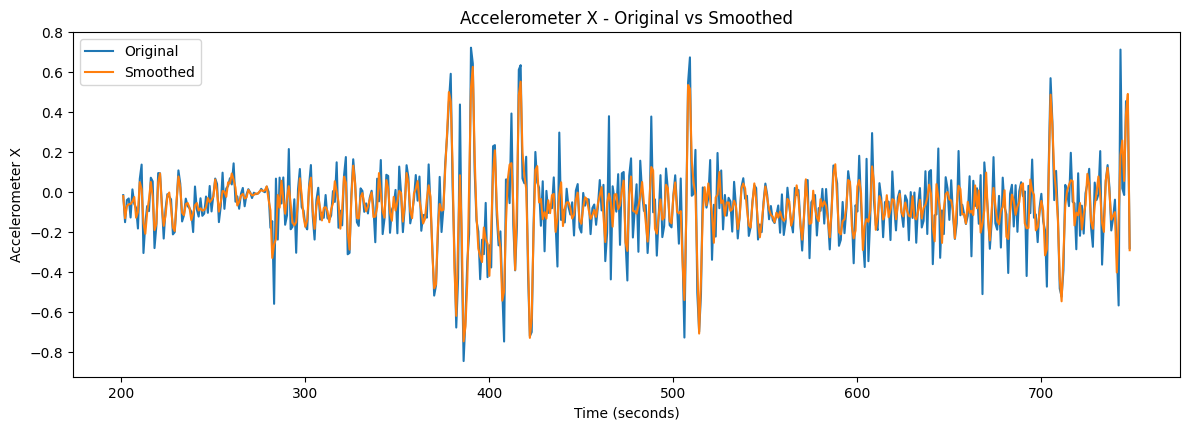
\includegraphics[width=\linewidth]{Figures/acc_x.png}
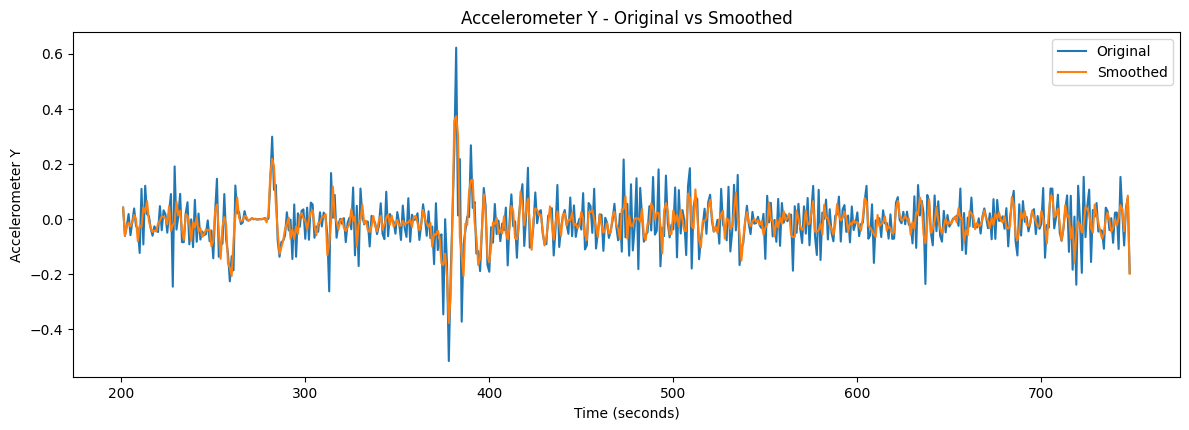
\includegraphics[width=\linewidth]{Figures/acc_y.png}
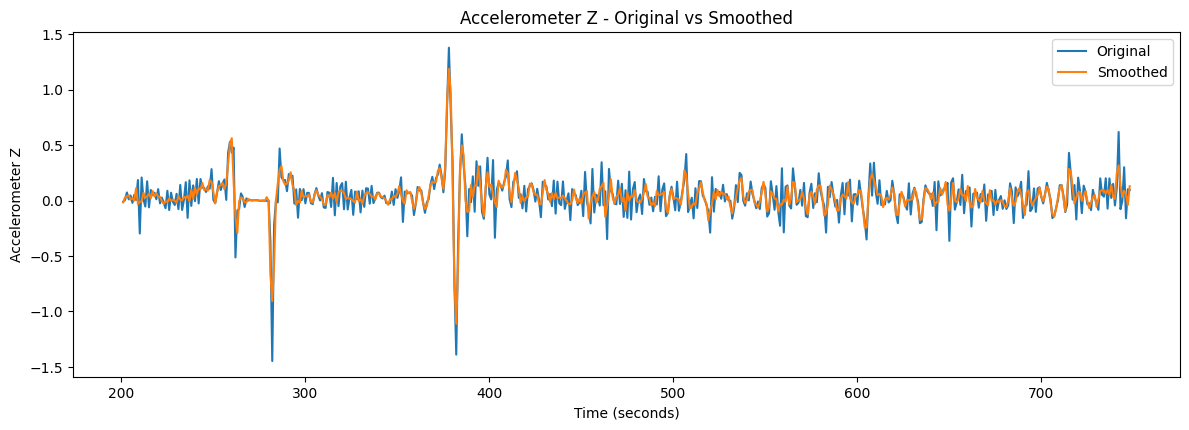
\includegraphics[width=\linewidth]{Figures/acc_z.png}
\caption{Graph showing smoothened data vs raw data over time.}
\label{fig:smooth}
\end{figure}
    \item \textbf{Feature Selection}: The data were reduced to a set of relevant features, including smoothed accelerometer data (\texttt{accelerometer\_x\_smooth}, \texttt{accelerometer\_y\_smooth}, \texttt{accelerometer\_z\_smooth}) and raw sensor readings (\texttt{accelerometer\_x}, \texttt{accelerometer\_y}, \texttt{accelerometer\_z}).
    \item \textbf{Labeling}: Labels were generated based on the difference between consecutive smoothed accelerometer readings. If the difference exceeded certain thresholds, the segment was labeled as ``bad quality'' (0), otherwise as ``good quality'' (1).
    \item \textbf{Training and Testing Split}: The pre-processed data were split into training and testing sets using an 80/20 ratio, ensuring that the model could be evaluated on unseen data.
\end{enumerate}

\subsection{Model Training}

Several machine learning models were implemented and trained using the pre-processed data:

\begin{enumerate}
    \item \textbf{Random Forest Classifier}: A robust ensemble model that uses multiple decision trees to improve classification accuracy.
    \item \textbf{Support Vector Machine (SVM)}: A model that maximizes the margin between data points of different classes, with a radial basis function (RBF) kernel.
    \item \textbf{K-Nearest Neighbors (KNN)}: A non-parametric model that classifies data points based on the majority vote of their nearest neighbors.
    \item \textbf{Logistic Regression}: A statistical model that estimates the probability of a binary outcome.
    \item \textbf{Neural Network}: A deep learning model with multiple layers, designed to capture complex patterns in the data. The network architecture included three dense layers with ReLU activation functions and a final softmax layer for classification.
\end{enumerate}

To address the class imbalance, the Synthetic Minority Over-sampling Technique (SMOTE) was applied to the training data. This technique generates synthetic samples to balance the class distribution, ensuring that the models were trained on a more representative dataset.

\subsection{Model Evaluation}

The models were evaluated using K-Fold Cross Validation, a technique that splits the data into multiple folds, ensuring that each fold serves as a validation set once. The average accuracy across folds was recorded for each model. Additionally, confusion matrices and classification reports were generated to assess the precision, recall, and F1-score of each model.

The neural network model was trained separately, using a 60-epoch training process with a validation split of 20\%. The performance of the neural network was evaluated on the test set, and predictions were compared with those from traditional machine learning models.

The results are available under the results section.

\subsection{Web Application Development}

A web application was developed using Flask to allow users to upload new sensor data, process it using the trained models, and visualize the results. The application provided the following functionalities:

\textbf{Data Upload}: Users could upload CSV files containing new sensor data for analysis.

\begin{figure}[H]
\centering
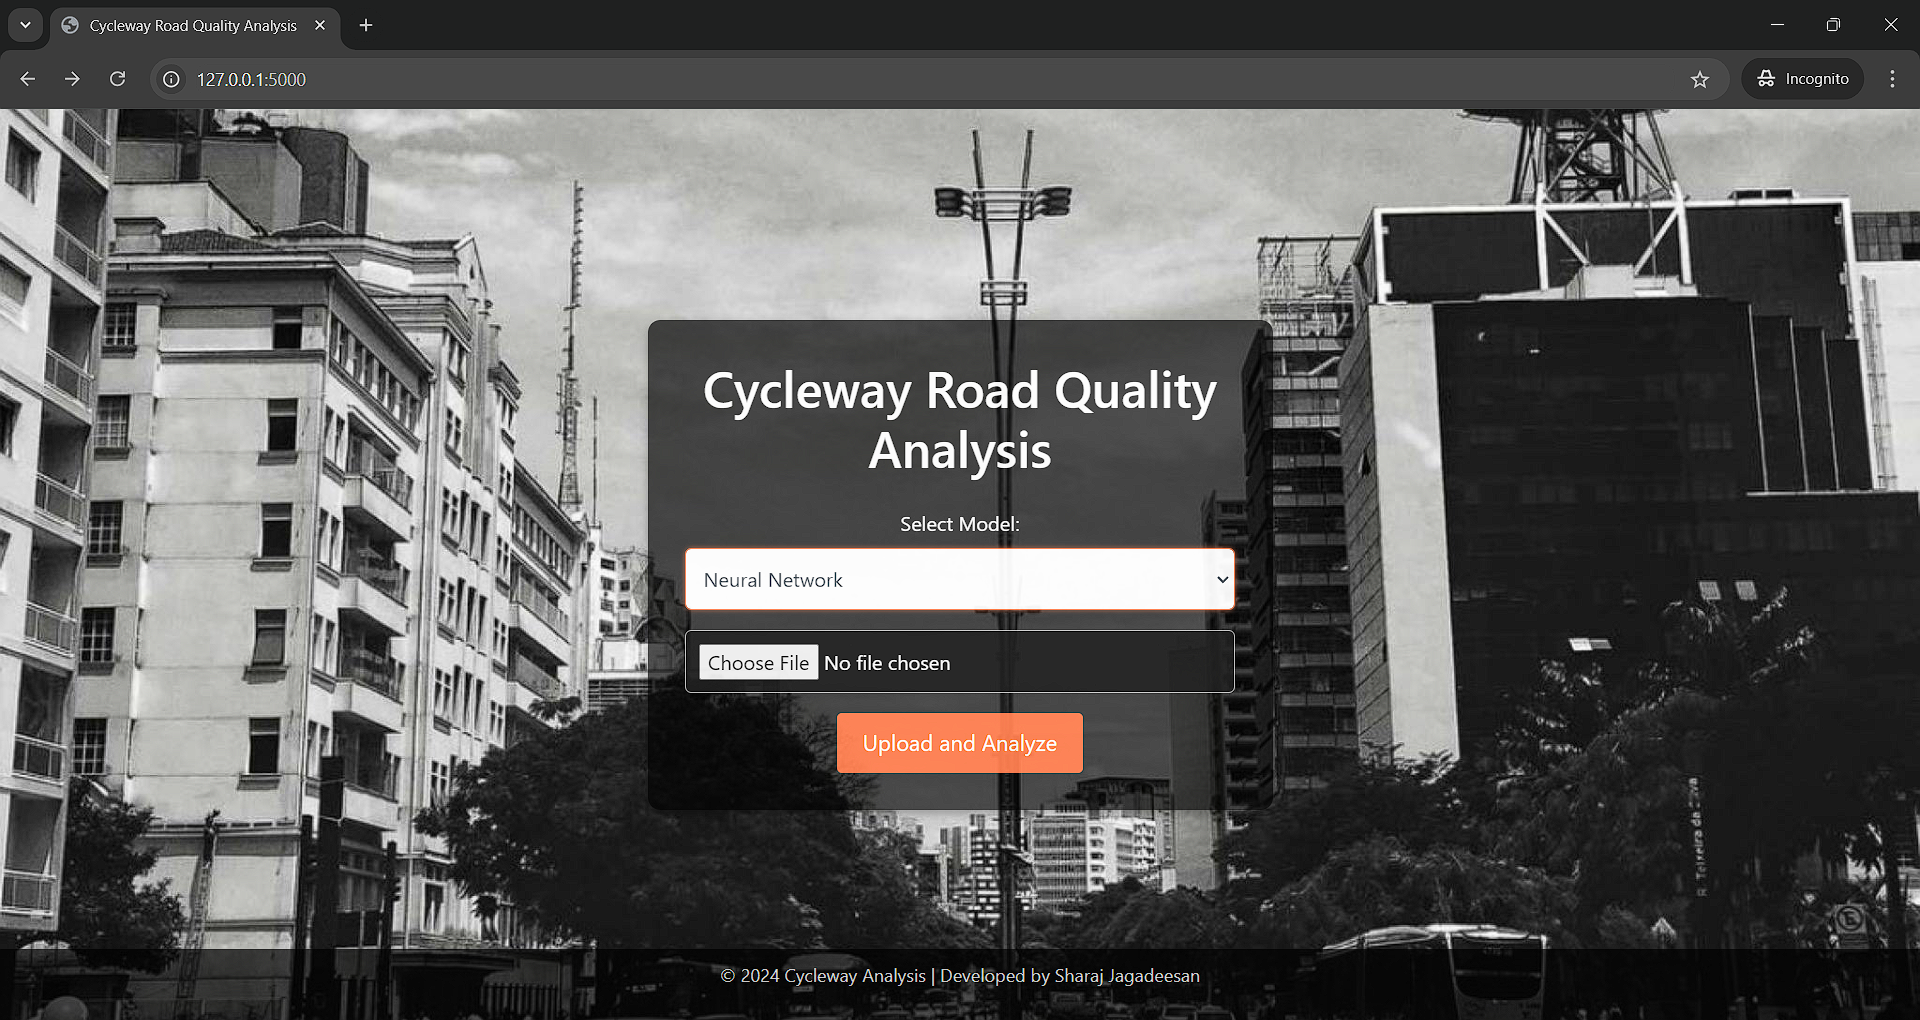
\includegraphics[width=\linewidth]{Figures/Screenshot1.png}
\caption{Web application interface for uploading CSV files for analysis.}
\label{fig:upload}
\end{figure}

\vspace{10pt}

\textbf{Model Selection}: The application allowed users to select from the trained models (Random Forest, SVM, KNN, Logistic Regression, Neural Network) for road quality prediction.

\vspace{10pt}

\textbf{Visualization}: The application generated maps with GPS coordinates, marking road segments predicted as ``bad quality'' and displaying corresponding images as shown in Figure \ref{fig:maps}. Additionally, graphs were created to visualize the smoothed accelerometer data, correlations between axes, and label distributions, as shown in Figure \ref{fig:graph}.

\begin{figure}[H]
\centering
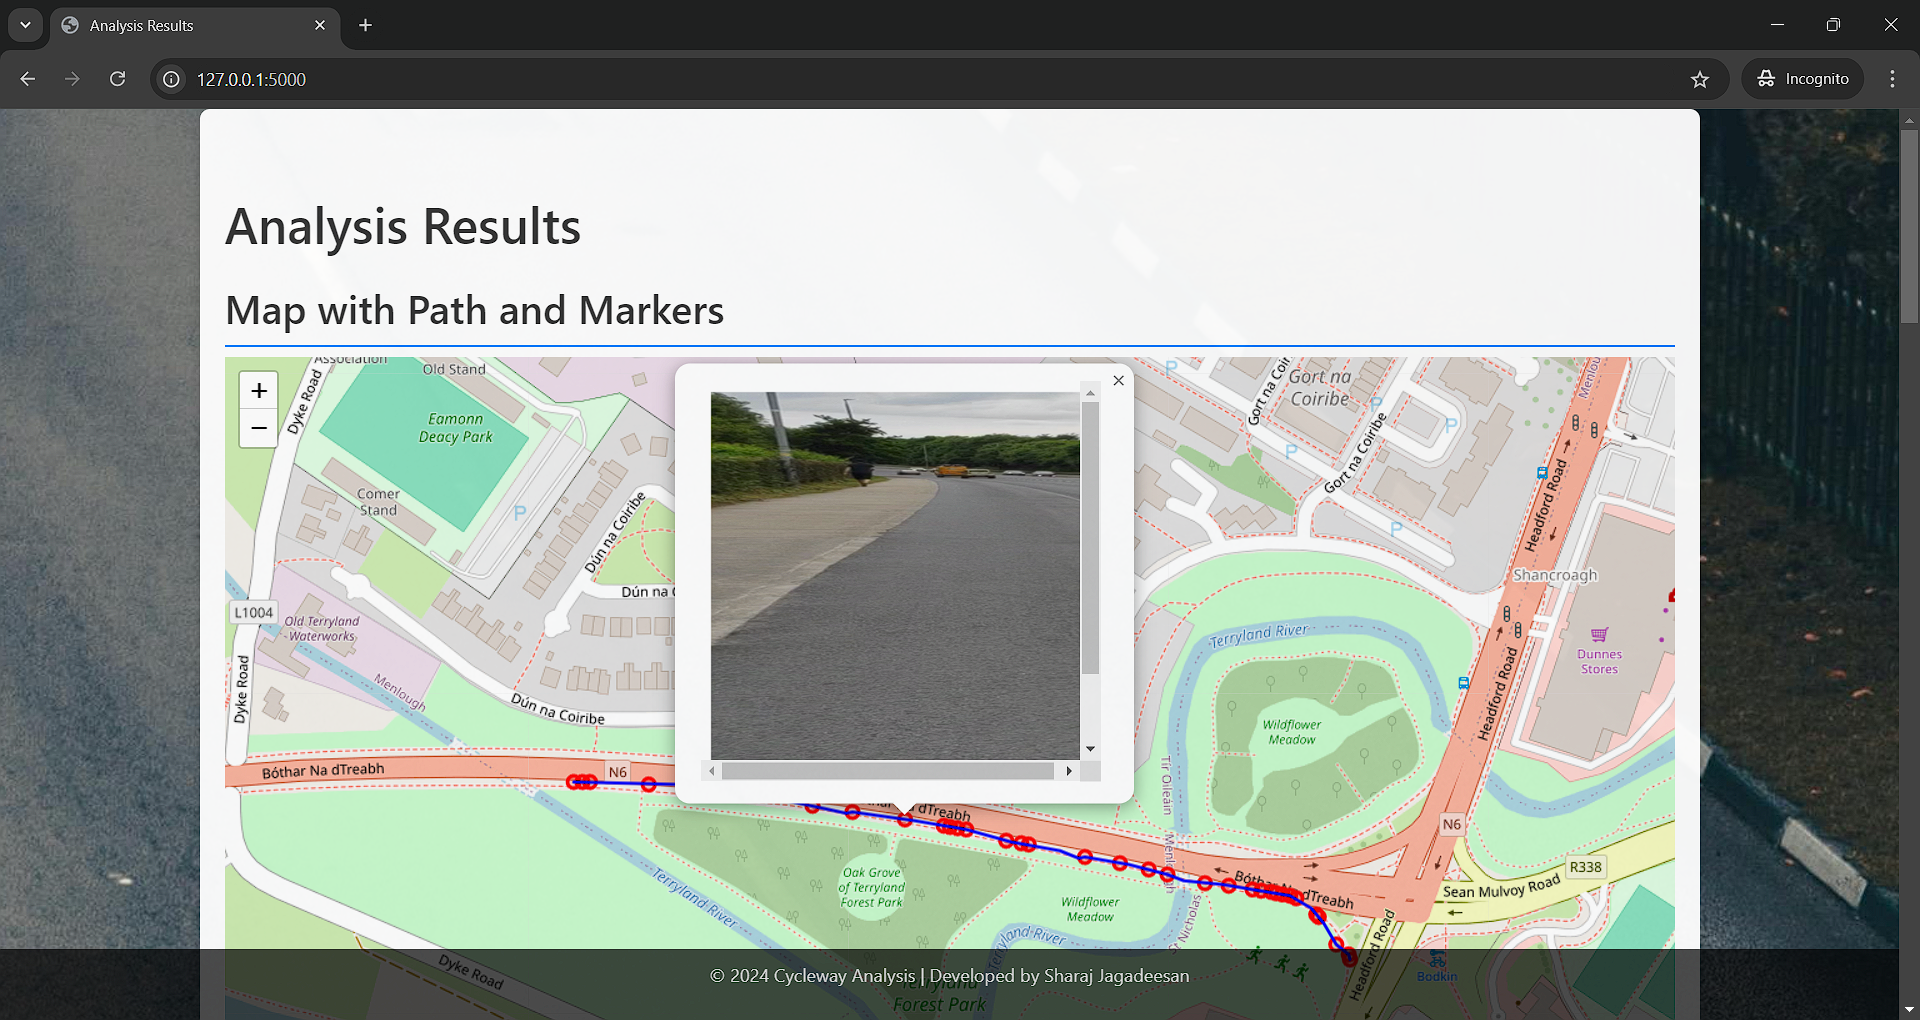
\includegraphics[width=\linewidth]{Figures/Screenshot2.png}
\caption{Map showing the road segments.}
\label{fig:maps}
\end{figure}

\begin{figure}[H]
\centering
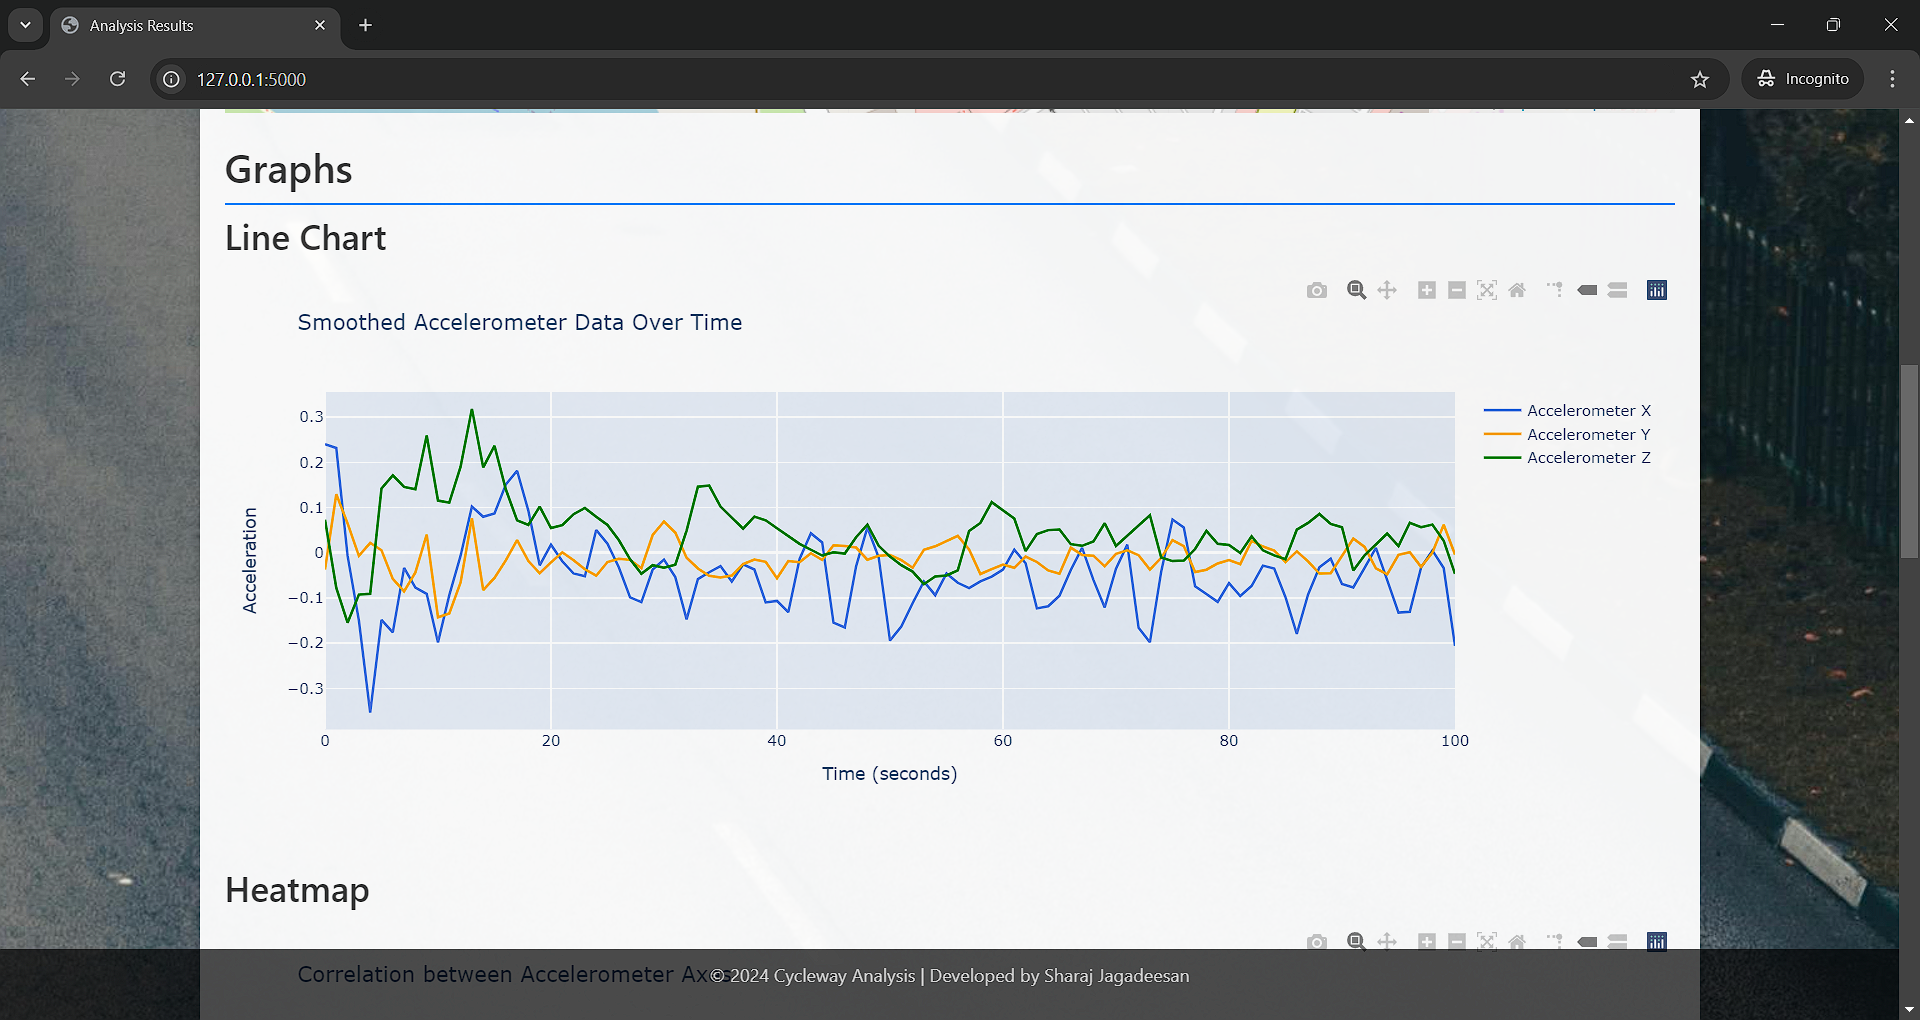
\includegraphics[width=\linewidth]{Figures/Screenshot3.png}
\caption{Graph displaying the accelerometer data over time.}
\label{fig:graph}
\end{figure}

\vspace{10pt}

\textbf{Prediction Results}: The application presented the prediction counts and percentages for ``good'' and ``bad'' road quality, providing an overview of the road conditions based on the uploaded data, as shown in Figure \ref{fig:charts}.

\begin{figure}[H]
\centering
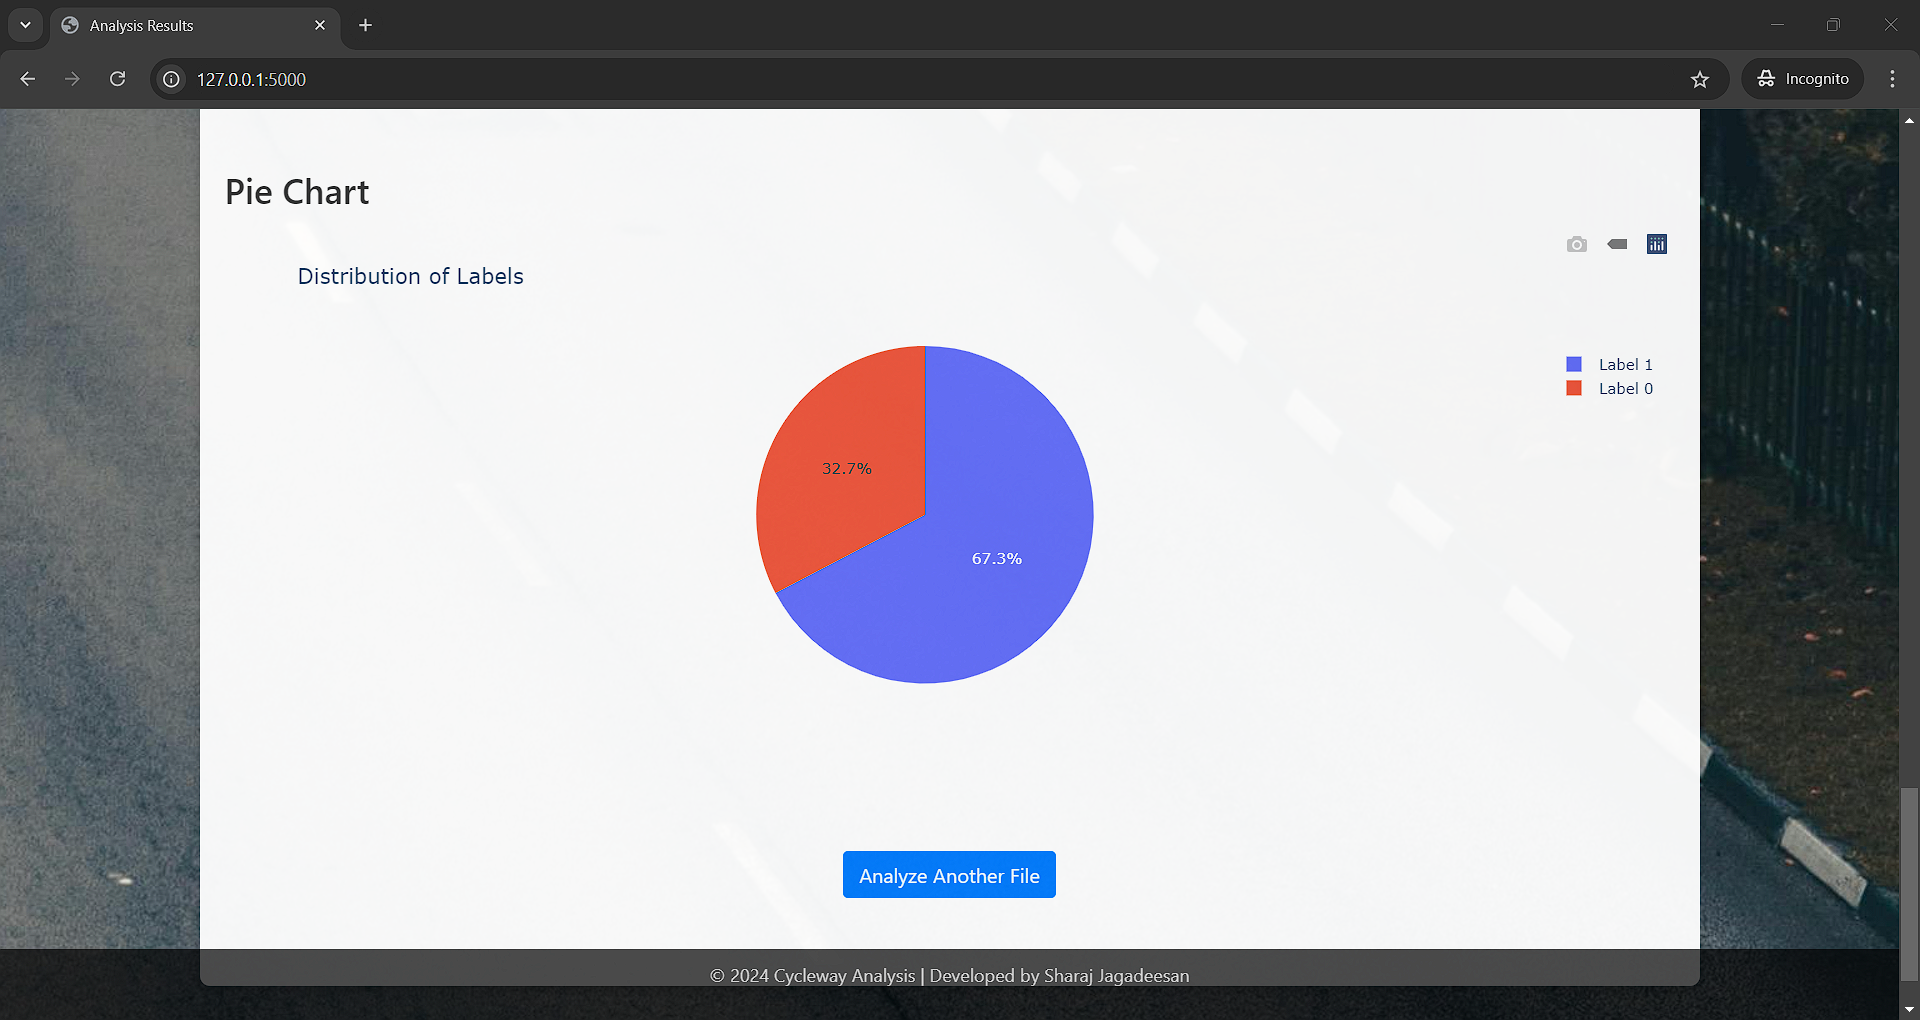
\includegraphics[width=\linewidth]{Figures/Screenshot6.png}
\caption{Pie chart showing the label counts.}
\label{fig:charts}
\end{figure}

The web application served as a practical tool for deploying the models and making the system accessible to end-users, facilitating real-time road quality assessment using mobile devices.

	
	\chapter{Results}
	\label{chap:results}
	
%%	Results first, using figures and tables, with little commentary and no interpretation.
	
%%	\noindent Then detailed analysis and interpretation.\\
	
%%	\textbf{Link experimental results to your \underline{research questions}} or hypotheses, e.g., ``The results in Table 3 clearly show that the answer to RQ2 is negative ...''.
The machine learning models were evaluated based on their accuracy in classifying road surface quality using the test dataset. The following table summarizes the accuracy of each model:

\begin{table}[h]
\centering
\begin{tabular}{|l|c|}
\hline
\textbf{Model} & \textbf{Accuracy (\%)} \\ \hline
Logistic Regression & 70.27 \\ \hline
K-Nearest Neighbours & 86.68 \\ \hline
Support Vector Machine & 77.62 \\ \hline
Random Forest & 91.54 \\ \hline
Neural Network & 94.55 \\ \hline
\end{tabular}
\caption{Accuracy of different machine learning models in detecting road surface quality.}
\label{tab:results}
\end{table}

Among the models tested, the \textbf{Neural Network} achieved the highest accuracy at \textbf{94.55\%}, followed closely by the \textbf{Random Forest} model with an accuracy of \textbf{91.54\%}. The \textbf{K-Nearest Neighbours (KNN)} model also performed well, achieving an accuracy of \textbf{86.68\%}. The \textbf{Support Vector Machine (SVM)} and \textbf{Logistic Regression} models achieved accuracies of \textbf{77.62\%} and \textbf{70.27\%}, respectively.

The results indicate that the Neural Network model is the most effective for the given task, likely due to its ability to capture complex patterns in the data through its deep learning architecture. The Random Forest model also demonstrated strong performance, benefiting from its ensemble approach to decision trees. In contrast, the Logistic Regression model, which is simpler and assumes a linear relationship between features, performed less effectively in this context.

\begin{figure}[h]
\centering
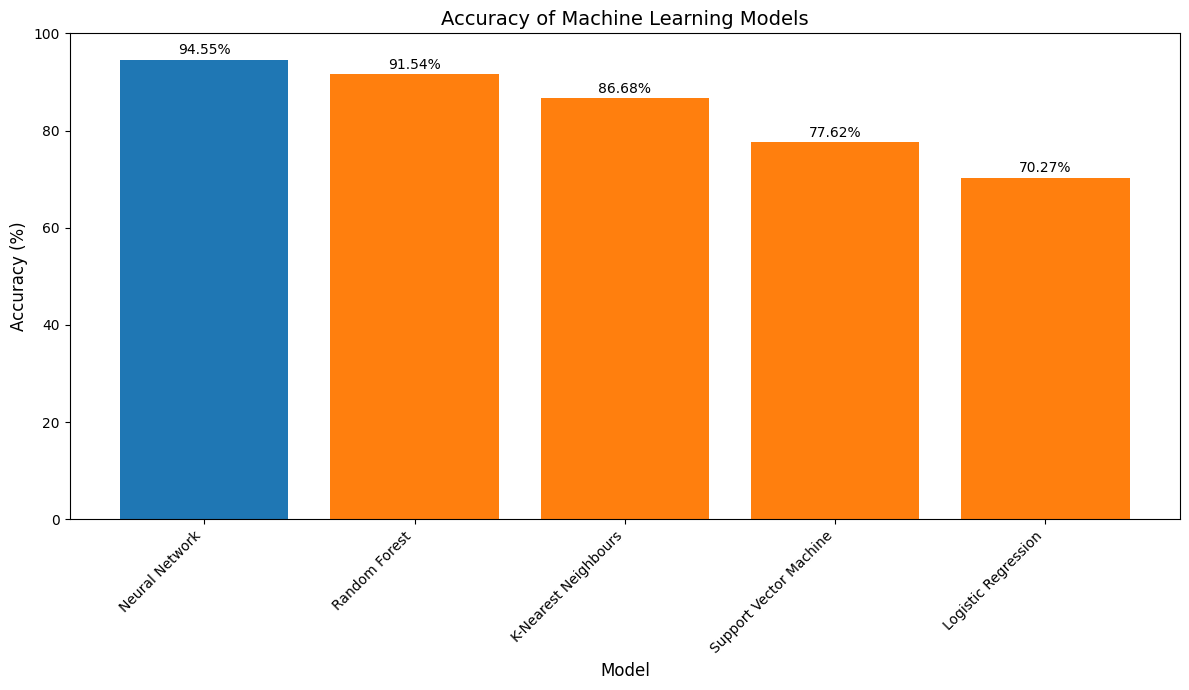
\includegraphics[width=\linewidth]{Figures/output.png}
\caption{Comparison of model accuracies for road surface quality detection.}
\label{fig:results}
\end{figure}

Figure \ref{fig:results} provides a visual comparison of the accuracies achieved by each model. This further highlights the superior performance of the Neural Network and Random Forest models in classifying road surface quality based on sensor data.
	\chapter{Conclusion}
	\label{chap:conclusion}
	
%%	Here you must zoom back out to evaluate the thesis itself. Mention its contributions and main results (in brief form), its limitations and weaknesses, and possible future work.
	This thesis successfully addressed the critical need for improved cycleway infrastructure management by creating a comprehensive data analytics tool designed specifically for evaluating road and cycleway quality. To process and classify sensor data collected from widely available devices like smartphones, the tool integrates advanced data analytics and machine learning models such as Random Forest, Support Vector Machine (SVM), K-Nearest Neighbors (KNN), Logistic Regression, and Neural Networks. This tool gives road development agencies and cyclists valuable insights by enabling real-time analysis and visualization of road conditions through an easy-to-use web application.

This work's main contributions are the index for measuring cycleway quality which was created the web-based platform for data analysis that was developed, and the machine learning models that were used to predict and visualize road quality. These contributions are significant because they close the gap found in the research, which was that the particular requirements of cycleway infrastructure management were not sufficiently met by the solutions that were already in place. The use of interactive visualizations, including maps, accelerometer data plots, correlation heatmaps, and label distribution charts, augments the tool's pragmatic usefulness and renders it an invaluable asset for enhancing bicycle safety and navigation and supporting road authorities' strategic planning and resource distribution.

This thesis does, however, suffer from certain drawbacks. The quality and diversity of the training data determine how accurate the machine learning models are, which may restrict the tool's usefulness to other situations or conditions that aren't covered by the data. Furthermore, the use of smoothed accelerometer data may mask finer details that are essential for precise classification, and the static model selection process may not always yield the best model for every dataset.

In order to improve the robustness of the models, future work should concentrate on addressing these limitations by expanding the dataset to include more diverse road conditions and geographic areas. The predictive performance may also be enhanced by putting in place an automated or ensemble-based model selection procedure. In order to enable live monitoring and analysis, real-time data processing and integration could also be explored. This would increase the tool's responsiveness and practicality. Lastly, adding more thorough analytics and ways for users to provide feedback would enhance the insights the tool offers even more and promote safer and more approachable urban settings.

In summary, this thesis makes a significant contribution to the field of cycleway infrastructure management by creating a workable and novel solution that makes use of cutting-edge machine learning and data analytics methods. Even though there is still room for improvement, the tool created for this project offers a strong foundation for further study and advancement and has the potential to have a big influence on how cycleways are improved and maintained in urban settings.


	%%%%%%%%%%%%%%%%%%%%%%%%%%%%%%%%%%%%%%%%%%%%%%%%%%%%%%%%%%%%%%%%%%%%%%%%%%%%%%%%
	%\bibliographystyle{plainnat}                  % to give author-year style
	\bibliographystyle{IEEEtranN} 
	\renewcommand{\bibname}{References}           % change default name Bibliography to References
	\bibliography{references}                     % BibTeX References file, references.bib
	\addcontentsline{toc}{chapter}{References}    % add References to TOC
	
	
	%%% uncomment if Appendices needed
	%\appendix
	%\chapter{Appendix-A-Title} 
	%\label{chap:appendix_a}
	
	%\chapter{Appendix-B-Title} 
	%\label{chap:appendix_b}
	
\end{document}
